\documentclass[12pt]{article}
\usepackage{graphicx}
\usepackage{float}
\usepackage{amsmath}
\title{Experiment 4: BCD Adder}
\author{Annirudh K P\\%
210070009}
\date{August 29, 2022}
\begin{document}

\maketitle

\section{Overview of the experiment}
\paragraph{}
In this experiment, we started working on more designs using structure modelling on VHDL. The problem statement of this experiment is to design a BCD Adder, using the 4-bit ripple carry adder already designed and other basic gates. The objective of this experiment was to understand the Quartus Design Flow, work with the Xen10 Board, and give us hands on experience over different technical glitches/problems we may face in this piece of software which has been made unwantedly hard.

\section{Experimental Set-up}

\subsection{Design Requirements}
\subsubsection{Prime Detector}
The BCD Adder takes in 2 BCD (0 to 9) numbers in binary form and adds them to spit out a 5 bit output.

Rules:
\begin{itemize}
\item Use 4-bit binary adder for initial addition.
\item Design a logic circuit to detect sum greater than 9.
\item One more 4-bit adder to add $(0110)_2$ in the sum if sum is greater than 9 or carry is 1.
\end{itemize}

\subsection{Design Schematics}
The following design schematics are shown for the BCD Adder 

\begin{figure}[H]
\centering
  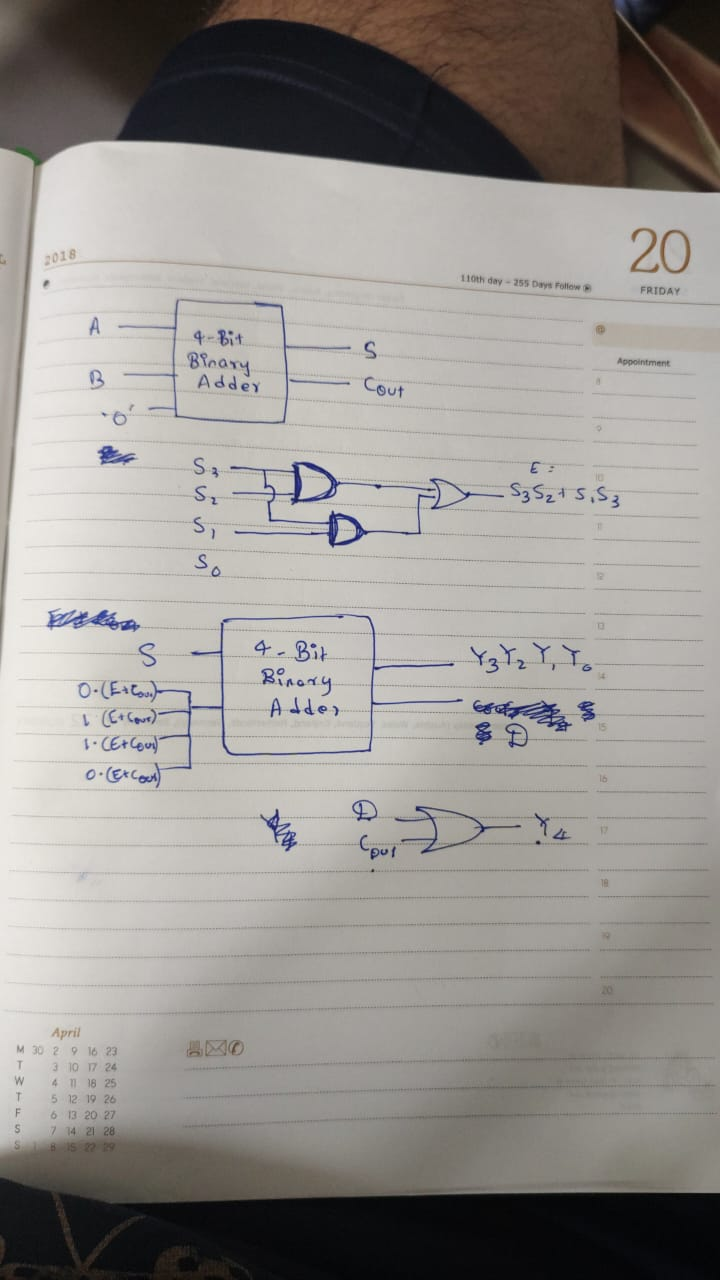
\includegraphics[scale=0.3]{Images/BCDAdder_Design.jpeg}
  \caption{BCD Adder Design}
\end{figure}

\subsection{Description of Components}
\subsubsection{Prime Detector}
\begin{verbatim}
library ieee;
use ieee.std_logic_1164.all;
library work;
use work.Gates.all;

entity OR_GATE  is
  port (A, B: in std_logic; OUTPUT: out std_logic);
end entity OR_GATE;

architecture Struct of OR_GATE is
	signal A_BAR, B_BAR : std_logic;
begin
  -- component instances
  NAND1: NAND_2 port map (A => A, B => A, Y => A_BAR);
  NAND2: NAND_2 port map (A => B, B => B, Y => B_BAR);
  
  -- final OR
  NAND3: NAND_2 port map (A => A_BAR, B => B_BAR, Y => OUTPUT);
end Struct;

library ieee;
use ieee.std_logic_1164.all;
library work;
use work.Gates.all;


entity HALF_ADDER1 is
	port (A, B: in std_logic; SUM, C0: out std_logic);
end entity HALF_ADDER1;

architecture Struct1 of HALF_ADDER1 is
	signal S1, S2, S3, S0 : std_logic;
begin
	--carry
	NAND1: NAND_2 port map (A => A, B => B, Y => S0);
	NAND2: NAND_2 port map (A => S0, B => S0, Y => C0);
	
	--sum
	NAND3: NAND_2 port map (A => A, B => B, Y => S1);
	NAND4: NAND_2 port map (A => A, B => S1, Y => S2);
	NAND5: NAND_2 port map (A => B, B => S1, Y => S3);
	NAND6: NAND_2 port map (A => S2, B => S3, Y => SUM);

end Struct1;

library ieee;
use ieee.std_logic_1164.all;
library work;
use work.Gates.all;

entity FULL_ADDER is
	port (A, B, CI: in std_logic; SUM, CO: out std_logic);
end entity FULL_ADDER;

architecture Struct2 of FULL_ADDER is
	signal S1, C1, C2 : std_logic;
	component HALF_ADDER1 is
		port (A, B: in std_logic; SUM, C0: out std_logic);
	end component HALF_ADDER1;
	component OR_GATE is
		port (A, B: in std_logic; OUTPUT: out std_logic);
	end component OR_GATE;
begin
	HA_1: HALF_ADDER1 port map (A => A, B => B, SUM => S1, C0 => C1);
	HA_2: HALF_ADDER1 port map (A => CI, B => S1, SUM => SUM, C0 => C2);
	OR_1: OR_GATE port map (A => C1, B => C2, OUTPUT => CO);
end Struct2;

library ieee;
use ieee.std_logic_1164.all;
library work;
use work.Gates.all;

entity XOR_GATE  is
  port (A, B: in std_logic; OUTPUT: out std_logic);
end entity XOR_GATE;

architecture Struct3 of XOR_GATE is
  signal S1, S2, S3 : std_logic;
begin
  -- component instances
  NAND1: NAND_2 port map (A => A, B => B, Y => S1);
  NAND2: NAND_2 port map (A => A, B => S1, Y => S2);
  NAND3: NAND_2 port map (A => B, B => S1, Y => S3);
  
  -- final XOR
  NAND4: NAND_2 port map (A => S2, B => S3, Y => OUTPUT);
  
end Struct3;

library ieee;
use ieee.std_logic_1164.all;
library work;
use work.Gates.all;

entity FourBitAdder  is
  port (M: in std_logic; A, B: in std_logic_vector(3 downto 0);
       	S: out std_logic_vector(3 downto 0); Cout: out std_logic); 
end entity FourBitAdder;

architecture Struct4 of FourBitAdder is
   signal Y1, Y2, Y3, Y4, Y5, Y6, Y7: std_logic;
	component XOR_GATE is
		port (A, B: in std_logic; OUTPUT: out std_logic);
	end component XOR_GATE;
	component FULL_ADDER is
		port (A, B, CI: in std_logic; SUM, CO: out std_logic);
	end component FULL_ADDER;
begin	
	XOR1: XOR_GATE port map (A => B(0), B => M, OUTPUT => Y1);
	FA_1: FULL_ADDER port map (A => Y1, B => A(0),  CI => M, SUM => S(0), 
		CO => Y2);
	XOR2: XOR_GATE port map (A => B(1), B => M, OUTPUT => Y3);
	FA_2: FULL_ADDER port map (A => Y3, B => A(1),  CI => Y2, SUM => S(1), 
		CO => Y4);
	XOR3: XOR_GATE port map (A => B(2), B => M, OUTPUT => Y5);
	FA_3: FULL_ADDER port map (A => Y5, B => A(2),  CI => Y4, SUM => S(2), 
		CO => Y6);
	XOR4: XOR_GATE port map (A => B(3), B => M, OUTPUT => Y7);
	FA_4: FULL_ADDER port map (A => Y7, B => A(3),  CI => Y6, SUM => S(3), 
		CO => Cout);
end Struct4;

library ieee;
use ieee.std_logic_1164.all;
library work;
use work.Gates.all;

entity BCDAdder  is
  port (A, B: in std_logic_vector(3 downto 0);
       	Y: out std_logic_vector(4 downto 0)); 
end entity BCDAdder;

architecture Struct5 of BCDAdder is
   signal S: std_logic_vector(3 downto 0); 
	signal Cout, E, D, D1, D2, E1: std_logic;
	component FourBitAdder  is
		port (M: in std_logic; A, B: in std_logic_vector(3 downto 0); 
		S: out std_logic_vector(3 downto 0); Cout: out std_logic); 
	end component FourBitAdder;
	
begin	
	FBIT_1: FourBitAdder port map (M => '0', A => A, B => B, S => S, 
		Cout => Cout);
	AND1: AND_2 port map (A => S(3), B => S(2), Y => D1);
	AND2: AND_2 port map (A => S(1), B => S(3), Y => D2);
	OR1: OR_2 port map (A => D1, B => D2, Y => E);
	OR2: OR_2 port map (A => E, B => Cout, Y => E1);
	FBIT_2: FourBitAdder port map (M => '0', A => S, B(0) => '0', 
		B(1) => E1, B(2) => E1, B(3) => '0', S => Y(3 downto 0), Cout => D);
	OR3: OR_2 port map (A => D, B => Cout, Y => Y(4));   
end Struct5;
\end{verbatim}

\section{Observations}
 
We get RTL simulation waveforms for corresponding to input and output which is given below and it shows required results.

\begin{figure}[H]
\centering
  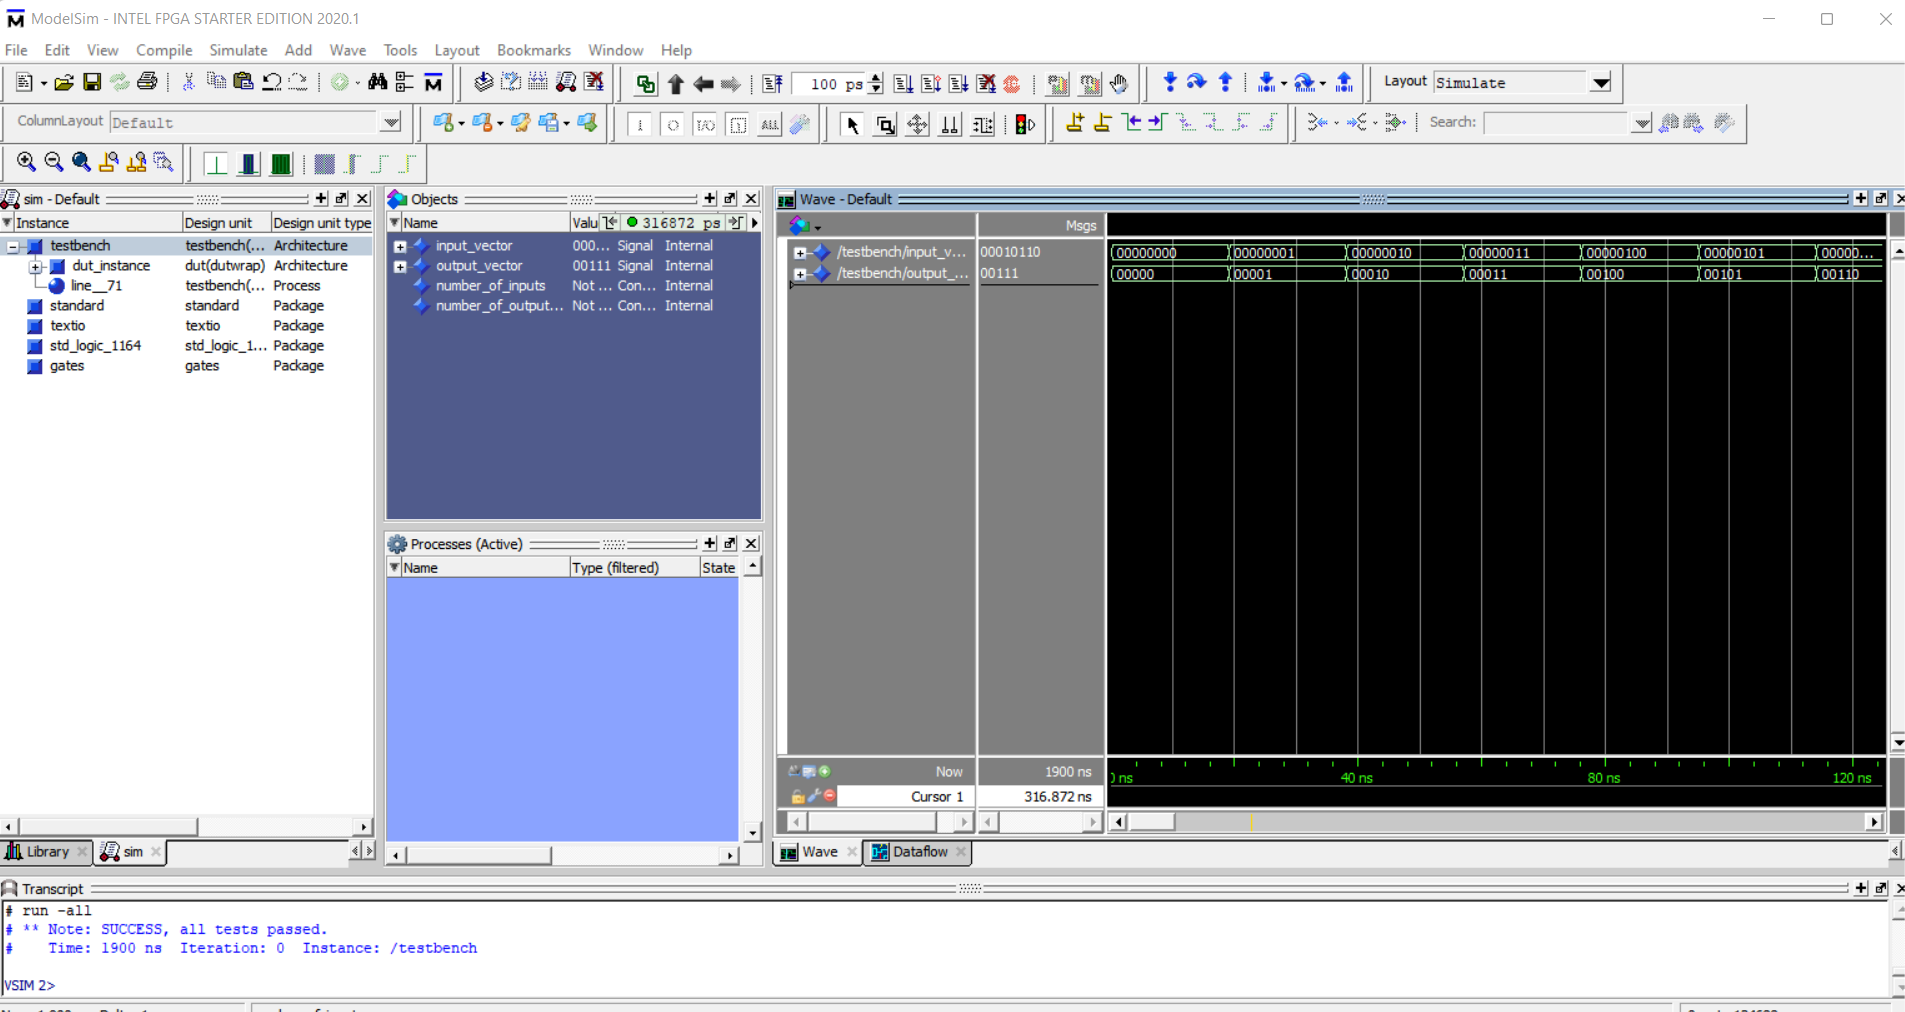
\includegraphics[scale=0.35]{Images/BCDAdder_RTLSimulation.png}
  \caption{BCD Adder RTL Simulation Waveform}
\end{figure}

Further the code (in form of .svf file) was flashed onto the Xen10 board, after the pins and LED were mapped accordingly. The output verified the working of the logic, and some example images are shown below.

\begin{figure}[H]
\centering
  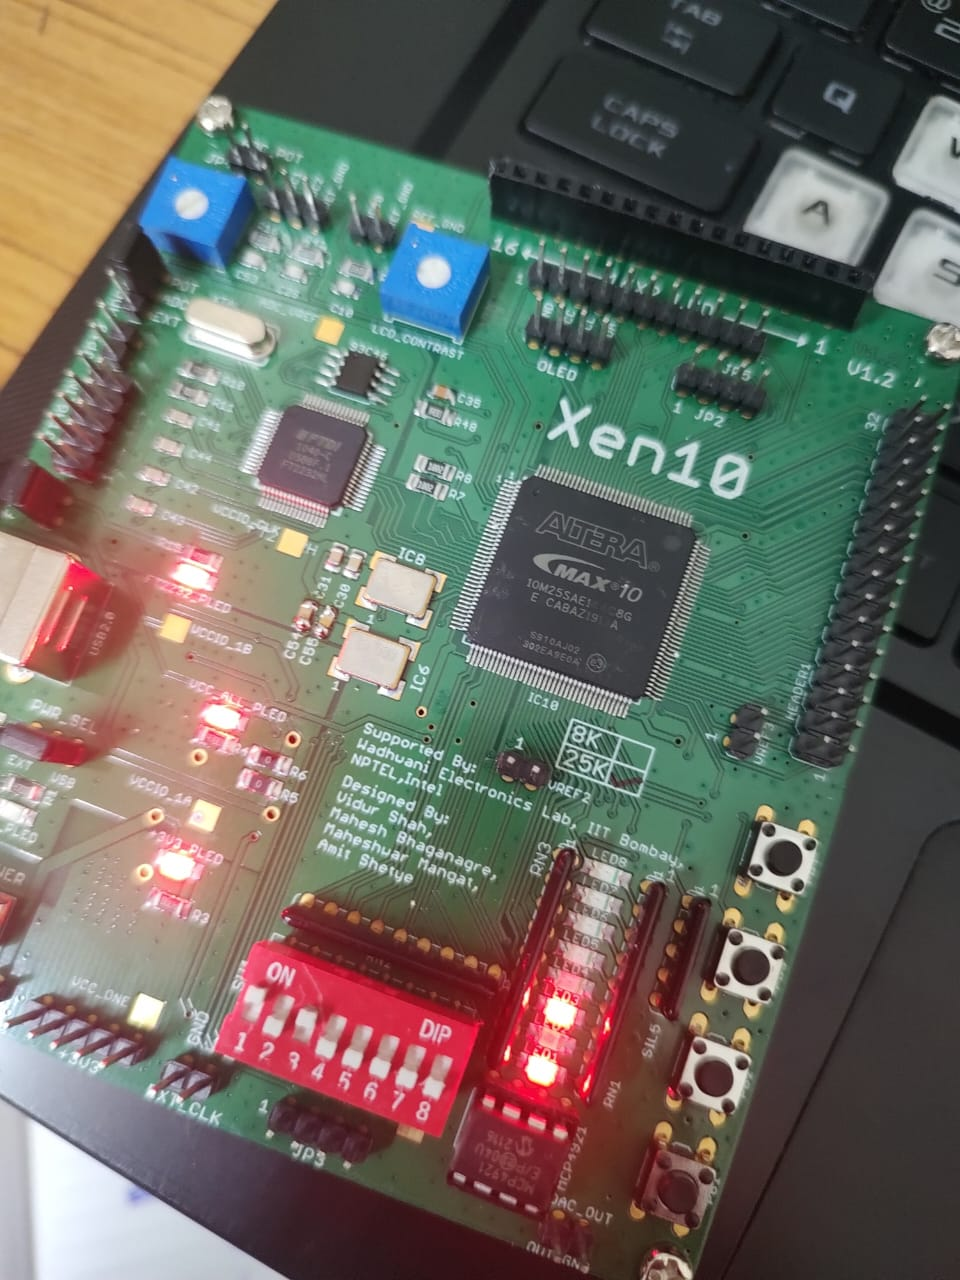
\includegraphics[scale=0.35]{Images/Trial01.jpeg}
  \caption{BCD Adder Example 1 - Xen10 Board}
\end{figure}

\begin{figure}[H]
\centering
  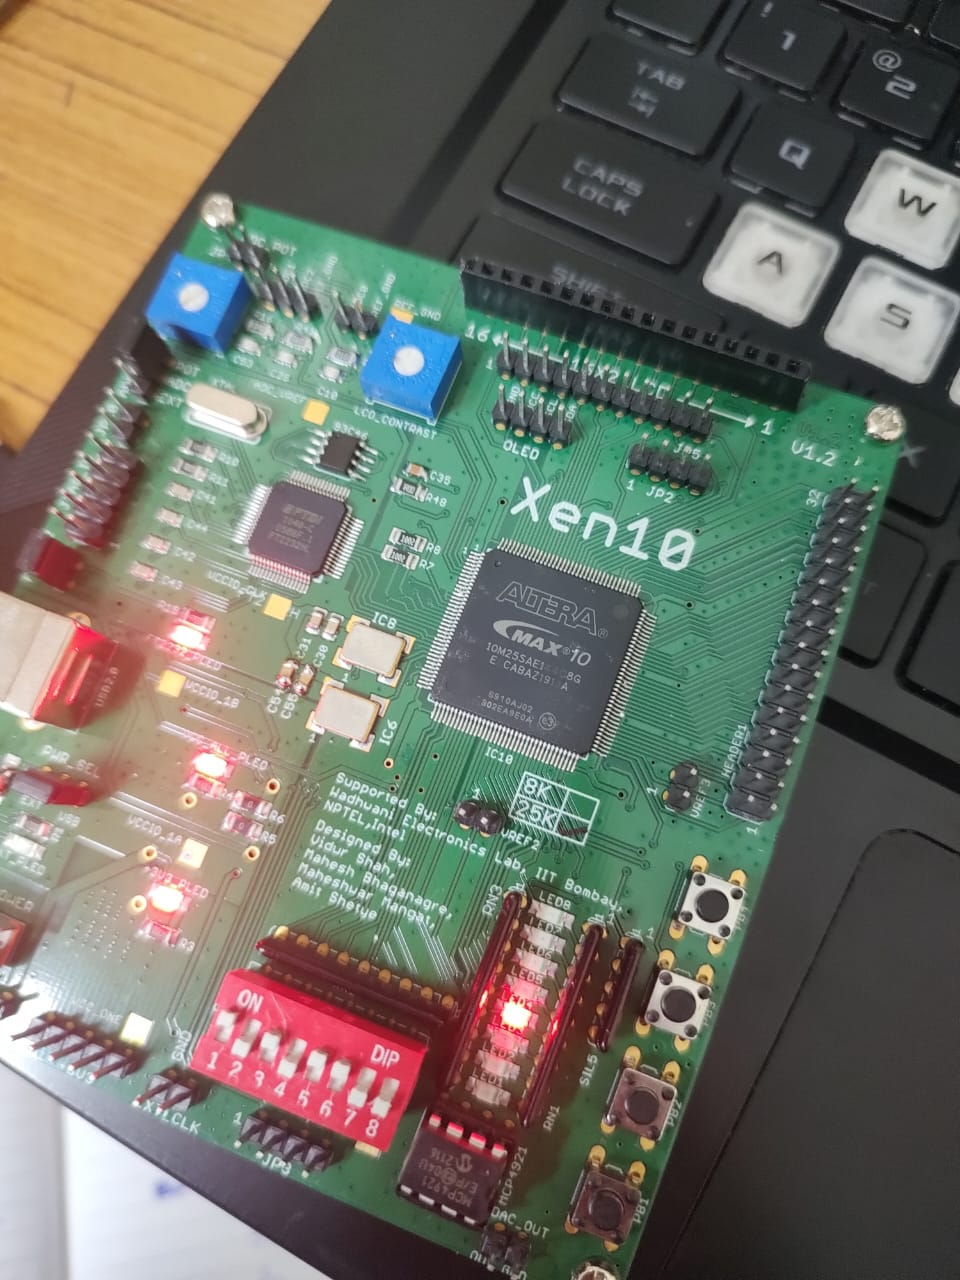
\includegraphics[scale=0.35]{Images/Trial02.jpeg}
  \caption{BCD Adder Example 2 - Xen10 Board}
\end{figure}

\begin{figure}[H]
\centering
  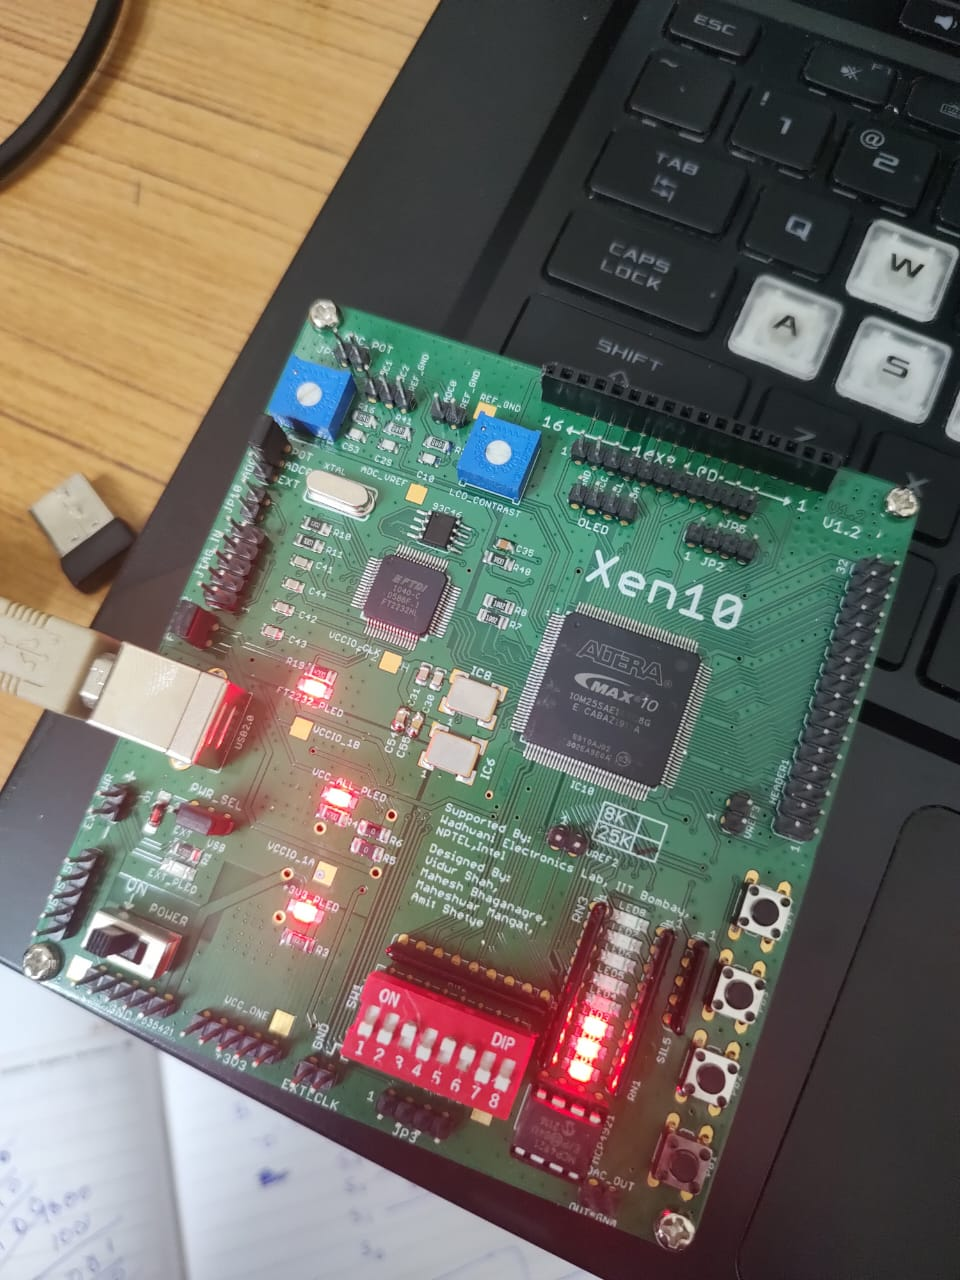
\includegraphics[scale=0.35]{Images/Trial03.jpeg}
  \caption{BCD Adder Example 3 - Xen10 Board}
\end{figure}

\end{document}